\section{A response instrument that can build a successor}
\label{sec:methods}

\subsection{Choose transfer before choosing confirmation}

The prospectively bounded development charter compares three mission families: resource scheduling,
repeated shortest paths, and grounded sparse-network analysis. It fixes four screen seeds, two sizes per
family, twelve repeat queries and one candidate mechanism per family, with at most 24 screen configurations.
The decision criteria precede the outcomes: a useful first result, genuinely fresh inputs, independently
checkable outputs, a distinct executable successor, a competent cheap builder, and a plausible unfavorable
shift. The selected domain permits at most six algorithm variants and three complete development campaigns.
Old confirmation cases remain historical results, not a newly declared development set.

Sparse-network analysis has a direct transfer hypothesis. The expensive common object is an operator;
the changing request is its applied load. A response instrument can avoid repeated factorization. A later
change in a small number of edges requires a different operator and can create a distinct instrument using
the first instrument's solve interface. These are standard numerical opportunities. They provide an honest
test of whether discovery, qualification, integration, persistence and upkeep erase the apparent benefit.

\subsection{Useful work and a separate numerical checker}

For $n$ nodes, let $e_i$ be the $i$th coordinate vector. An edge $a=(u,v)$ has incidence vector
$b_a=e_u-e_v$ and positive conductance $w_a$. With positive diagonal grounding $G$, define
\begin{equation}
 A=G+\sum_{a\in E} w_a b_a b_a^{\mathsf T},\qquad A x=f.
 \label{eq:network}
\end{equation}
The output $x$ is the response to a new load $f$. In the synthetic computational model it can be interpreted
as node potentials or a grounded steady-state response; no physical network was built or calibrated.
The useful result includes node values, edge flows, current input identity and numerical check evidence.

The checker is implemented separately from matrix assembly and the solver. It accumulates each node's
ground term and incident edge flows directly from the supplied edge list, using compensated summation.
It also compares dissipated energy with applied work:
\begin{align}
 r_i &=g_i x_i+\sum_{(i,j)\in E} w_{ij}(x_i-x_j)-f_i,\\
 \mathcal E(x)&=\sum_i g_i x_i^2+\sum_{(u,v)\in E}w_{uv}(x_u-x_v)^2.
\end{align}
Qualification requires both a normalized maximum residual and normalized energy discrepancy no larger
than $10^{-9}$. The schema rejects nonfinite data, nonpositive conductances, invalid endpoints and grounding
below $0.1$. The accepted domain has at most 65,536 nodes and 1,000,000 supplied edges; the experiment uses
the smaller frozen sizes specified in its protocol.

Positive grounding and conductance make $A$ symmetric positive definite. Hence a residual is relevant to
the fixed numerical problem: for the exact solution $x^\star$, $A(x-x^\star)=r$, and
$\|x-x^\star\|_2\leq\|r\|_2/g_{\min}$. This algebraic bound does not validate a physical interpretation,
source annotations or real demand. The second energy check is a useful consistency check, not an independent
real-world oracle. The separate implementation reduces shared-code error while retaining the limitations of
one commissioned team, one host and a common mathematical specification.

\subsection{Start with an available specialist}

The initial service uses the justified native COLAMD sparse factorization and retains its already-computed
factor as a byproduct of the accepted result. There is no second artificial builder charge for the same factor.
The comparison set includes native sparse direct factorization and preconditioned conjugate gradient;
ordinary warm starts and conventional factor reuse are permitted. SciPy's \artifact{splu} invokes SuperLU
and returns a reusable solve object; its documented column orderings include COLAMD and minimum-degree
variants \citep{scipy117splu}. The conjugate-gradient path uses a diagonal preconditioner, the previous
accepted solution as an allowed initial guess, a fixed tolerance and a finite iteration limit
\citep{scipy117cg}. The experiment does not handicap the direct method by erasing legitimate previous work.
The frozen comparison distinguishes standalone specialist performance from total workbench and custody cost.

The software relies on established SciPy algorithms \citep{virtanen2020scipy}. No new linear solver,
factorization, low-rank identity or uniquely agentic advantage is claimed. The contribution lies in the
causal mission sequence, executable inheritance, protected resource accounts, complete comparisons and
explicit decision boundaries.

\subsection{Mission A and the retained parent}

Mission A delivers a checked solution on $A$ and the native factor used to produce it. Candidate parent capability $F$ stores an exact operator
identity, dependency versions, permutations and sparse factors, exposing
\begin{equation}
 F:\ f\longmapsto x\approx A^{-1}f.
\end{equation}
It is a method for responding to new loads, not a stored answer to A. Its native construction cost is already
charged to A; recording it again as separate research would double count. Retention in the research catalogue requires a checked output and an explicit
scope; scientific validity, prospective product adoption and recovery of investment remain different decisions.

The asset interface binds dimensions, operator hash, chosen ordering and dependency versions. Its lifecycle
cost includes construction, current-output checking, integration, retrieval, storage and maintenance. Portable
arrays are stored without executable pickle objects. Reload verifies the byte receipt, metadata, array shapes,
permutations and triangular structure before using sparse triangular solves \citep{scipy117triangular}.
The native live factor and portable restored factor may have different execution costs; their mathematical
interface alone does not establish equal operational performance.

\subsection{Mission B: fresh work, actual use and a real predecessor}

Each B request supplies a new right-hand side on the same accepted operator. Before reuse, the adapter
rechecks operator identity and scope, then records actual parent calls. Every returned response receives
the current edge-list checker. The distinct successor requirement is selected from the actual accepted
preceding B output: edges are ordered by absolute realized flow, with a fixed index tie-break. The chosen
positive conductance increments and the preceding input, solution and receipt digests enter the successor
identity. A separately generated baseline cannot stand in for this accepted state.

This state-dependent rule is itself frozen. It makes the input to construction depend on useful completed
work without allowing a failed candidate to redefine the acceptance test. Across treatments, the design
retains actual prior-state provenance and reports any resulting requirement differences; apparently identical
ancestry labels do not establish equivalent tasks.

\subsection{Mission C: construct a distinct update instrument}

For $k$ changed edges with positive increments $\delta_j$, form
\begin{equation}
 U=\big[\sqrt{\delta_1}b_{a_1},\ldots,\sqrt{\delta_k}b_{a_k}\big],\qquad
 A'=A+UU^{\mathsf T}.
\end{equation}
The constructor invokes the parent on the columns of $U$, obtaining $W=F(U)$. It then retains
$S=I+U^{\mathsf T}W$ and exposes the distinct operator
\begin{equation}
 H(f)=F(f)-W S^{-1}U^{\mathsf T}F(f)\approx (A')^{-1}f.
 \label{eq:woodbury}
\end{equation}
This is the established Sherman--Morrison--Woodbury construction \citep{hager1989}. The original parent
cannot correctly answer an arbitrary load on $A'$ by itself. Its execution helps construct $H$, and each
fresh use of $H$ again calls the parent. The original operator, exact increments, actual accepted B receipt,
parent identity and dependencies are bound to the successor. Construction-call and delivery-call counts
are recorded separately.

\begin{figure}[ht]\centering
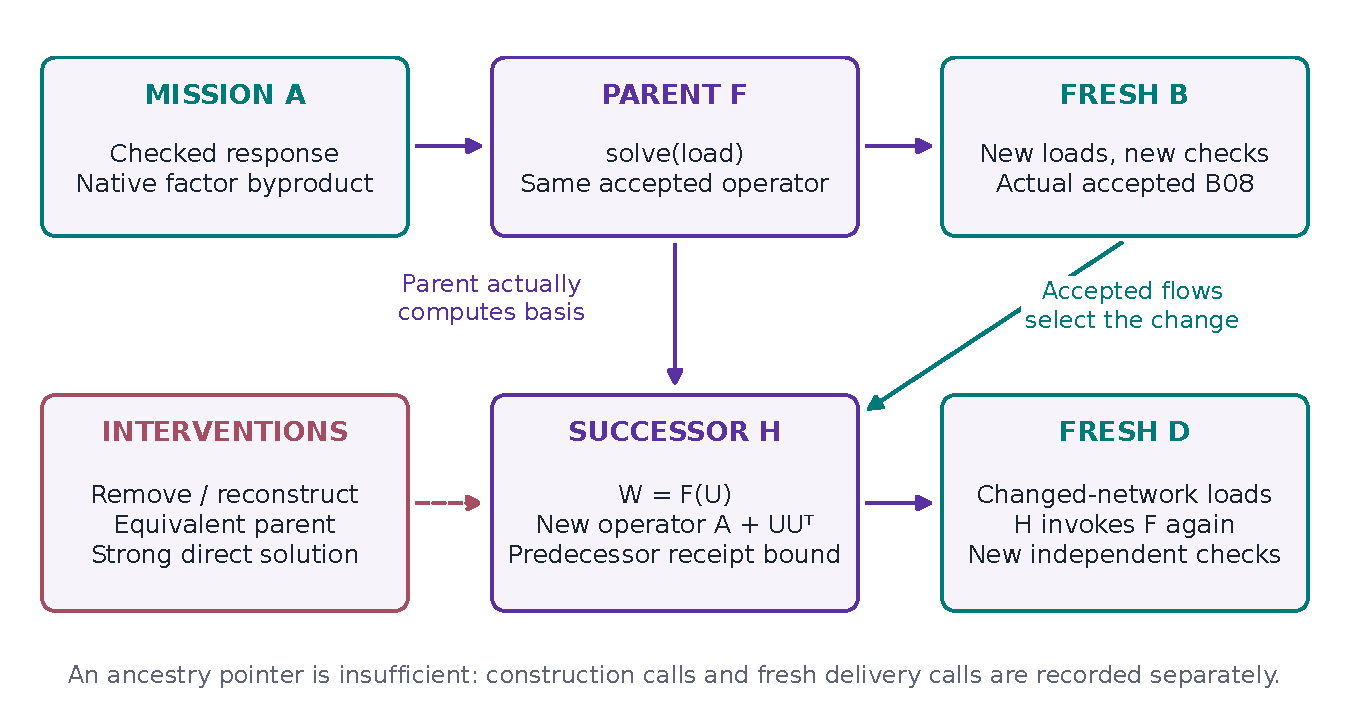
\includegraphics[width=\linewidth]{figures/causal-lineage.pdf}
\caption{An operational lineage. The accepted B response determines the changed requirement; the retained parent actually computes the response basis used to construct the new instrument. Fresh D requests use the changed operator and receive new checks. Counterfactual treatments intervene on the executable parent, not merely its ancestry label.}
\label{fig:lineage}
\end{figure}

The implementation retains an incumbent or uses native refactorization when the registered scope policy
declines the update. A grounding change invalidates both earlier operator scopes. Nonpositive edge
conductance is refused as unsupported. Such cases are preserved as outcomes; they are not silently replaced
by easier confirmation inputs. A failed construction must leave a competent service alternative available.

\subsection{Causal comparisons and three different improvements}

\textbf{Execution improvement} asks whether fresh accepted work costs less or achieves more at the same
resource limit. \textbf{Construction improvement} asks whether retaining $F$ makes building or qualifying
$H$ better than reconstructing the parent, independently constructing an equivalent asset, or using a
strong parent-free solver. \textbf{Discovery improvement} would require a separately evaluated improvement
to the search for such methods. It is not inferred from the first two.

The inherited, reconstructed, equivalent, native-refactor and equally enabled conventional treatments retain
the same input rights and reasonable optimization opportunities. Conventional reuse may invoke the identical
method and erase any named-controller advantage. Parent removal allows reconstruction; the parent-free
specialist remains entitled to solve $A'$ directly. A parent-use count establishes that an interface was
invoked. Its causal value requires the corresponding outcome/cost contrast. A cheaper exact reconstruction
comparison alone cannot establish practical adoption against a stronger direct alternative.

\subsection{Separate validity, adoption and investment}

For asset $a$, let $C_{\rm build}$ be construction and initial qualification cost, $m$ the prospective number
of applicable uses, $c_a$ current cost per qualified use including upkeep, and $c_\star$ the best available
alternative. A simple break-even condition is
\begin{equation}
 m(c_\star-c_a)>C_{\rm build},\qquad c_\star>c_a.
 \label{eq:breakeven}
\end{equation}
The actual decision uses the registered uncertainty and quality conditions; this expression explains why
recurrence matters. Once construction is sunk, marginal adoption instead compares future burdens.
The provisional research-use rule compares frozen development medians for the construction kernel plus
the declared remaining solves: $1.20\,\widehat C_{\rm candidate}<\widehat C_{\rm native}$.
This applies a 20\% surcharge to the candidate forecast, equivalent to requiring more than a 16.7\% reduction
relative to the native forecast. It does not
predict complete persistence, checking, transport or maintenance cost, and therefore is not product admission.
The protected confirmation applies the stronger whole-workflow product rule: every required output must
qualify, the paired stream interval must support at least a 5\% CPU benefit over native refactorization,
and the workflow must satisfy the registered 10\% noninferiority margin against equally enabled conventional
reuse. Otherwise product status remains HOLD. Passing a cheaper kernel comparison cannot substitute for
this complete-system gate.
Investment recovery must additionally charge exploration, rejected variants, complete checking, integration,
maintenance, recovery and attributable human effort. Unknown human durations and monetary cost remain unknown.
A candidate can be numerically valid and worth adopting prospectively while its full research investment
remains unrecovered. Conversely, valid inheritance can be an expensive liability.
